\section{Results}

\subsection{Classification accuracy}

We take particular interest in the accuracy of each subject's best-case task pair, as we predict this task pair would acheive the best discrimatory power \textcolor{red}{[Why is it so? This should be motivated well in advance, e.g. in introduction and method sections}.  We achieved excellent best-case performance overall, and maintained an estimated x\% accuracy among all subjects, even at recording lengths of 1/2 second.

% TODO: table of best-case at different bin-sizes and times?

Surprisingly, classification was better than chance even at a bin size of y, meaning that each feature vector in the training and testing sets contained only y features.

{\bf copy/ paste from email May 9 by Nick}

{\bf Q. 2.}

    By the way, I generated the average classification performance per subject directly in the spreadsheet. In most cases, we see little decrease in performance vs. bins. Although the accuracy is always above gambling (50\%), some subjects are clearly harder to classify than others. This is maybe an interesting result to discuss further.


% TODO: something about BCI illiteracy!

\begin{figure}
\begin{center}
%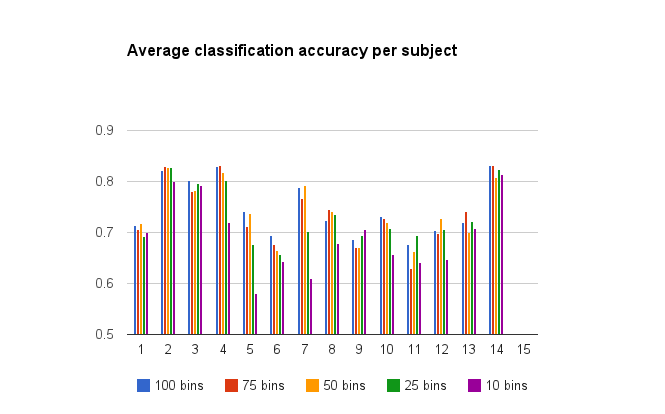
\includegraphics[width=6in]{Figures/avg_classification_accuracy_per_subject.png}
\caption{ }
\label{ }
\end{center}
\end{figure}


i'm wondering if there are a few outlier tasks here - like, a few tasks on which we get very low classification accuracy, dragging down the average
 

{\bf Q. 3.} Related to the average classification accuracy per task pair (second Figure), the difference between task pairs is striking. It seems that all pairs involving ``color" rate high, as well as ``finger" and ``base". However, it's hard to distinguish between ``finger" and ``base" ! I recall that the "color" task is longer than others. I guess it can be a reason for this result \textcolor{red}{\bf [Did you make any correction to take into account only the same sample size, i.e., max 10 seconds?]}. I attached an updated chart with all x-axis labels.

\begin{figure}
\begin{center}
%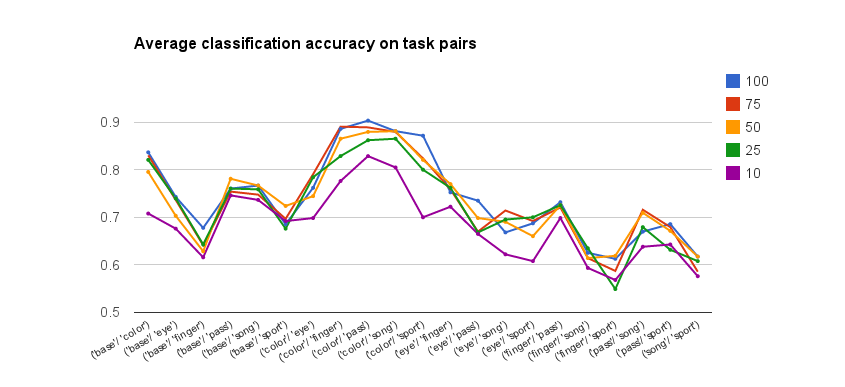
\includegraphics[width=6in]{Figures/avg_classification_accuracy_taskpairs.png}
\caption{ }
\label{ }
\end{center}
\end{figure}


{\bf Q. 5.} I also recall that we have discussed that it would be great to look how long (in seconds) it take to properly classify. Concretely, we have more or less 10 seconds per sample (at the exception of the ``color" task as far as I remember). So instead of classifying on the binned probability density function (pdf) build from an averaging power spectra over 10 seconds, what happens if we classify based on pdfs built on averaging power spectra on 1,2,3,...., and then 10 seconds instead ?




\subsection{Performance}

% TODO: figure of performance versus speed

% TODO: report regression between performance and speed

% TODO: regression on testtime as well?